\documentclass[a4paper]{article}
\usepackage{geometry}
\usepackage{graphicx}
\usepackage{natbib}
\usepackage{amsmath}
\usepackage{amssymb}
\usepackage{amsthm}
\usepackage{paralist}
\usepackage{epstopdf}
\usepackage{tabularx}
\usepackage{longtable}
\usepackage{multirow}
\usepackage{multicol}
\usepackage[hidelinks]{hyperref}
\usepackage{fancyvrb}
\usepackage{algorithm}
\usepackage{algorithmic}
\usepackage{float}
\usepackage{paralist}
\usepackage[svgname]{xcolor}
\usepackage{enumerate}
\usepackage{array}
\usepackage{times}
\usepackage{url}
\usepackage{fancyhdr}
\usepackage{comment}
\usepackage{environ}
\usepackage{times}
\usepackage{textcomp}
\usepackage{caption}
\usepackage{multirow}
\graphicspath{ {./} }


\urlstyle{rm}

\setlength\parindent{0pt} % Removes all indentation from paragraphs
\theoremstyle{definition}
\newtheorem{definition}{Definition}[]
\newtheorem{conjecture}{Conjecture}[]
\newtheorem{example}{Example}[]
\newtheorem{theorem}{Theorem}[]
\newtheorem{lemma}{Lemma}
\newtheorem{proposition}{Proposition}
\newtheorem{corollary}{Corollary}


\floatname{algorithm}{Procedure}
\renewcommand{\algorithmicrequire}{\textbf{Input:}}
\renewcommand{\algorithmicensure}{\textbf{Output:}}
\newcommand{\abs}[1]{\lvert#1\rvert}
\newcommand{\norm}[1]{\lVert#1\rVert}
\newcommand{\RR}{\mathbb{R}}
\newcommand{\CC}{\mathbb{C}}
\newcommand{\Nat}{\mathbb{N}}
\newcommand{\br}[1]{\{#1\}}
\DeclareMathOperator*{\argmin}{arg\,min}
\DeclareMathOperator*{\argmax}{arg\,max}
\renewcommand{\qedsymbol}{$\blacksquare$}

\definecolor{dkgreen}{rgb}{0,0.6,0}
\definecolor{gray}{rgb}{0.5,0.5,0.5}
\definecolor{mauve}{rgb}{0.58,0,0.82}

\newcommand{\Var}{\mathrm{Var}}
\newcommand{\Cov}{\mathrm{Cov}}

\newcommand{\vc}[1]{\boldsymbol{#1}}
\newcommand{\xv}{\vc{x}}
\newcommand{\Sigmav}{\vc{\Sigma}}
\newcommand{\alphav}{\vc{\alpha}}
\newcommand{\muv}{\vc{\mu}}

\newcommand{\red}[1]{\textcolor{red}{#1}}
\renewcommand\vec[1]{\boldsymbol{#1}}

\def\x{\mathbf x}
\def\y{\mathbf y}
\def\w{\mathbf w}
\def\v{\mathbf v}
\def\E{\mathbb E}
\def\V{\mathbb V}
\def\R{\mathbb R}
% TO SHOW SOLUTIONS, include following (else comment out):
\newenvironment{soln}{
    \leavevmode\color{blue}\ignorespaces
}{}


\hypersetup{
%    colorlinks,
    linkcolor={red!50!black},
    citecolor={blue!50!black},
    urlcolor={blue!80!black}
}

\geometry{
  top=1in,            % <-- you want to adjust this
  inner=1in,
  outer=1in,
  bottom=1in,
  headheight=3em,       % <-- and this
  headsep=2em,          % <-- and this
  footskip=3em,
}


\pagestyle{fancyplain}
\lhead{\fancyplain{}{Homework 4}}
\rhead{\fancyplain{}{CS 760 Machine Learning}}
\cfoot{\thepage}

\title{\textsc{Homework 4}} % Title

%%% NOTE:  Replace 'NAME HERE' etc., and delete any "\red{}" wrappers (so it won't show up as red)

\author{
\red{MADHUSHREE  NIJAGAL} \\
\red{9084490524}\\
} 

\date{}

\begin{document}

\maketitle 


\textbf{Instructions:} 
Use this latex file as a template to develop your homework.
Submit your homework on time as a single zip (containing the pdf and the code) file to Canvas. Please, check Piazza for updates about the homework. It is recommended that you use Python for your solutions. You are allowed to use the libraries {\tt {\tt numpy}}, {\tt matplotlib}, {\tt pandas} and {\tt pytorch}.
\section{Questions (50 pts)}
\begin{enumerate}
\item (10 Points)
Suppose the world generates a single observation $ x\sim$ multinomial($\vec \theta$), where the parameter vector $ \vec \theta = (\theta_1, \ldots , \theta_k)$ with $\theta_i\geq 0$ and $\sum_i^k\theta_i = 1$. Note $x \in \{1, \ldots, k\}$. You know $\theta$ and want to predict $x$. Call your prediction $\hat x$. What is your expected 0-1 loss: 
\[\E[1\{\hat{x} \neq x\}]\] 
using the following two prediction strategies respectively? Prove your answer. 
\begin{enumerate}
    \item (5 pts) Strategy 1: $\hat x \in \mathrm{argmax}_x\theta_x $, the outcome with the highest probability.  \\
    \begin{soln}  
	As given in the problem statement, we know the value of $\theta$ and from the strategy we can imply that the value of $\theta$ is maximum. When $\theta$ is maximum, we have $P(\hat x = x)$ and the loss is 0 and when we have values of $\theta$ less than the maximum value we have $P(\hat x \neq x)$ and the loss is 1. That is when x is misclassified ($\hat x \neq x$), the loss is 1 and 0 when correctly classified ($\hat x = x)$. Therefore we can write the expected loss function \[\E[1\{\hat{x} \neq x\}]\] as:
	\begin{center}
	 	  = $\sum x* P(x)$ = $1*P(\hat x \neq x) + 0*P(\hat x = x) $ \\
		  = $1*P(\hat x \neq x) = 1 - P(\hat x = x) = 1 - \theta_{max} $ \\
	\end{center}
     \end{soln}
    \item (5 pts) Strategy 2: You mimic the world by generating a prediction $ \hat{x}\sim$ multinomial($\vec \theta$). (Hint: your randomness and the world’s randomness are independent) 
    \begin{soln} \\As mentioned above, the loss function can be written as a function of all the values that are misclassified, that is when loss is 1 and values that are correctly classified, that is when loss is 0. Here the values of $\hat x$ and x are independent. Therefore the expected loss function can be written as \[\E[1\{\hat{x} \neq x\}]\] 
    \begin{center}
      		= $\sum x* P(x)$ = $1*P(\hat x \neq x) + 0*P(\hat x = x) $ \\
      		= 1 - $[P(\hat x = 1, x = 1) + P(\hat x = 2, x = 2) + ..... + P(\hat x = k, x = k)]$ \\
     		= 1 - $[{\theta_1}^{2} + {\theta_2}^{2} + ..... + {\theta_3}^{2}]$ \\
     		= 1 - $\sum_{i=1}^k \theta_i^{2}$
    \end{center}
    \end{soln}
\end{enumerate}

\item (10 points) Like in the previous question, the world generates a single observation $ {x}\sim$ multinomial($\vec \theta$). Let $c_{ij}\geq 0$ denote the loss you incur, if $x = i$ but you predict $\hat x = j$, for $i, j \in \{1, \ldots, k\}$. $c_{ii} = 0$ for all $i$. This is a way to generalize different costs on false positives vs false negatives from binary classification to multi-class classification. You want to minimize your expected loss: 
\[\E[c_{x\hat x}]\] 
Derive your optimal prediction $\hat x$. 
	\begin{soln} 
		\\We are given that the x = i and $\hat x$ = j and associated cost is $c_{ij} >= 0$ and if x = $\hat x = i$, the associated cost is $c_{ii} = 0$. We can represent the same information in the following matrix as: 
		\[\begin{bmatrix} 
			0 & c_{12} & c_{13} \\
			c_{21} & 0 & c_{23}\\
			c_{31} & c_{32} & 0 \\
		\end{bmatrix} \]
		Therefore the loss function can be represented as $\E[c_{x\hat x}]$ = $\sum_{j=1}^k \sum_{i=1}^k c_{ij} \theta_{i} \theta_{j}$.\\
		The $\theta_{i}$ and $\theta_{j}$ are the probabilities of x and $\hat x$ respectively. To minimize the expected loss, we need to minimize the function by finding the smallest value of $c_{ij}$ for every i value and vary j, the function is represented as: \\
		$\hat x \in \mathrm{argmin}_j (\sum_{i=1}^k \theta_i c_{ij})$
	\end{soln}

\item (30 Points)The Perceptron Convergence Theorem shows that
the Perceptron algorithm will not make too many mistakes
as long as every example is ``far'' from the separating hyperplane of the target halfspace.
In this problem, you will explore a {\em variant} of the Perceptron algorithm
and show that it performs well (given a little help in the form of a good initial hypothesis)
as long as every example is ``far'' (in terms of angle)
from the separating hyperplane of the \textit{current hypothesis}.

Consider the following variant of Perceptron:

\begin{itemize}

\item Start with an initial hypothesis vector $\vec w = \vec w^{\text{init}}$.

\item Given example $\vec x \in \mathbb{R}^n$,
predict according to the linear threshold function $\vec w \cdot \vec x \geq 0$.

\item Given the true label of $\vec x$, update the hypothesis vector $\vec w$ as follows:

\begin{itemize}

\item If the prediction is correct, leave $\vec w$ unchanged.

\item If the prediction is incorrect, set $\vec w \leftarrow \vec w - (\vec w \cdot \vec x) \vec x$.

\end{itemize}

\end{itemize}

So the update step differs from that of Perceptron shown in class 
in that $(\vec w \cdot \vec x) \vec x$ (rather than $\vec x$) is added or subtracted to $\vec w$.
(Note that if $\|\vec x\|_2 = 1$, then this update causes vector $\vec w$ to become orthogonal to $\vec x$,
i.e., we add or subtract the multiple of $x$ that shrinks $\vec w$ as much as possible.)

Suppose that we run this algorithm on a sequence of examples that are labeled
according to some linear threshold function $\vec v \cdot \vec x \geq 0$
for which $\|\vec v\|_2 = 1$. Suppose moreover that

\begin{itemize}

\item Each example vector $\vec x$ has $\|\vec x\|_2 = 1$;

\item The initial hypothesis vector $\vec w^{\text{init}}$
satisfies $\|\vec w^{\text{init}}\|_2 = 1$ and
$\vec w^{\text{init}} \cdot \vec v \geq \gamma$
for some fixed $\gamma > 0$;

\item Each example vector $\vec x$ satisfies
$\frac{|\vec w \cdot \vec x|}{\|\vec w\|_2} \geq \delta$,
where $\vec w$ is the current hypothesis vector when $\vec x$ is received.
(Note that for a unit vector $\vec x$, this quantity $\frac{|\vec w \cdot \vec x|}{\|\vec w\|_2}$
is the cosine of the angle between vectors $\vec w$ and $\vec x$.)

\end{itemize}

Show that under these assumptions, the algorithm described above
will make at most $\frac{2}{\delta^2} \ln(1/\gamma)$ many mistakes.
\end{enumerate}

	\begin{soln} 
	So we are given that for every true value of x, if the prediction is incorrect we have $\vec w$ updated by $\vec w - (\vec w \cdot \vec x) \vec x$ \\
	The convergence upper bound proof: \\
	Therefore for every mistake the update done can be represented as below: $\vec w_{t+1} = \vec w_t - (\vec w_t \cdot \vec x)\vec x $ \\
	Squaring both the sides we get: \\
	\begin{center}
	 $\|\vec w_{t+1}\|^{2}$ = ${\|\vec w_{t} - (\vec w \cdot \vec x) \vec x\|}^{2}$ \\
	 = $ {\|\vec w_{t} - (\vec w \cdot \vec x) \vec x)\|}^{T}\|\vec w_{t} - (\vec w \cdot \vec x) \vec x\|$ \\
	\end{center}
	 Expanding the above we get: \\
	 \begin{center}
	  $\|\vec w_{t+1}\|^{2} =  {\|\vec w_{t}\|}^{2} - 2 {\|\vec w_{t}(\vec w \cdot \vec x) \vec x\|}^2 + {\|(\vec w \cdot \vec x) \vec x\|}^{2}$ \\
	  $\|\vec w_{t+1}\|^{2} = {\|\vec w_{t}\|}^{2} -  |{\vec w \cdot \vec x}|$ ; since we have  $\|\vec x\|_2 = 1$ \\
	 $\frac{|\vec w_{t+1}|^{2}}{{\|\vec w_t\|}^{2}} = 1 - \frac{|\vec w \cdot \vec x|^{2}}{{\|\vec w\|}^{2}} \leq 1 - \delta^2$ \\
	 \end{center}
	 After $m_t$ mistakes the update to $\vec w$ changes to: \\
	  \begin{center}
	 $\|\vec w_{t+1}\|^2 \leq {(1 - \delta^2)}^{m_t}$ --$>$ Proof 1 \\
	 \end{center}
	 The convergence lower bound proof: \\
	 $\vec w^{init} = 1$ \\
	 $\vec w_{t+1} = \vec w^{init} - (\vec w \cdot \vec x)\vec x$ \\
	 $\vec w_{t+1} - \vec w^{init} = - (\vec w \cdot \vec x)\vec x$ \\
	 After $m_t$ mistakes we have: \\
	  \begin{center}
	  $\vec w_{t+1} - \vec w^{init} =  \sum_{i = 0}^{m_t}- (\vec w \cdot  \vec x)\vec x$ \\
	  $\vec w_{t+1} - \vec w^{init} = - \sum_{i = 0}^{m_t} (\vec w \cdot \vec x)\vec x$ \\
	  \end{center}
	  Taking the dot product of $\vec v$ on both sides: \\
	  \begin{center}
	  $\vec w_{t+1} \cdot \vec v - \vec w^{init} \cdot \vec v = - \sum_{i = 0}^{m_t} (\vec w \cdot \vec x)\vec x \cdot \vec v$ \\
	  $\vec w_{t+1} \cdot \vec v =  - \sum_{i = 0}^{m_t} (\vec w \cdot \vec x)\vec x \cdot \vec v + \vec w^{init} \cdot \vec v$ \\
	   \end{center}
	 We have $\vec w^{init} \cdot \vec v >= \gamma$ and $\|\vec v\|_2 = 1$ \\
	  \begin{center}
	  $\|\vec w_{t+1}\| >= \gamma $---$>$ Proof 2
	  \end{center}
	  Combining both Proof 1 and Proof 2, we have 
	  \begin{center}
	  ${(1 - \delta^2)}^{m_t} >= \gamma^2$
	 \end{center}
	 Taking ln on both sides: \\
	  \begin{center}
	  $m_t ln(1 - \delta^2) >= 2 ln \gamma$ \\
	  We know that $- ln(1 - x) >= x$ and replacing it the above equation we get: \\
	  $-m_t {\delta}^2 >= 2 ln(\gamma)$ \\
	  $-m_t >= 2 ln(\gamma) / {\delta}^2 $ \\
	  Simplifying, we get $m_t <= 2 / {\delta}^2 *ln(1/\gamma) $ \\
	  
	  \end{center}
	\end{soln}
\section{Programming (60 pts)}
In this exercise, you will derive, implement back-propagation for a simple neural network, and compare your output with some standard library’s output. Consider the following 3-layer neural network. 
\[\vec y = \vec f(\vec x) = \vec g(\vec W_2 \vec \sigma (\vec W_1 \vec x))\] 
Suppose $\vec x \in \R^d,\vec W_1 \in \R^{d_1\times d}$ and $\vec W_2 \in \R^{k\times d_1}$ i.e., $f : \R^d\mapsto \R^k$, Let $\vec \sigma (\vec z) = [\sigma(\vec z_1), \ldots , \sigma(\vec z_n)]$ for any $\vec z\in \R^n$ where $\sigma(t)=\frac{1}{1+\exp(-t)}$ is the sigmoid (logistic) activation function and $\vec g(\vec z)_i = \frac{\exp(\vec z_i)}{\sum_{i=1}^k  \exp(z_i)}$ is the softmax
function. Suppose that the true pair is $(\vec x, \vec y)$ where $\vec y \in \{0, 1\}^k$ with exactly one of the entries equal to 1 and you are working with the cross-entropy loss function given below, 
\[
L(\vec x,\vec y) = -\sum_{i=1}^k 
\vec y \log (\hat{\vec y})\;. 
\]
\begin{enumerate}
    \item Derive backpropagation updates for the above neural network. (10 pts )
    \begin{soln}
    \\We are given cross entropy loss function is given by $L(\vec x,\vec y) = -\sum_{i=1}^k 
\vec y \log (\hat{\vec y})\;. $ \\
	Some of the notations can be defined as: \\
	\begin{center}
	$z^{(1)} = W^{(1)}x$ \\
	$a^{(1)} = \sigma(z^{(1)})$\\
	$z^{(2)} = W^{(2)}a^{(1)}$ \\
	$a^{(2)} = \hat y = softmax(z^{(2)})$ \\
	\end{center}
	To derive the back-propagation update, we need to calculate the partial derivative of the loss function with respect to the $W^{(2)}$\\
	By chain rule we can express the partial derivative as:\\
	\begin{center}
	$\frac{\partial L}{\partial W^{(2)}}$ = $\frac{\partial L}{\partial \hat y}$ $\frac{\partial \hat y}{\partial z^{(2)}}$ $\frac{\partial z^{(2)}}{\partial W^{(2)}}$\\
	$\frac{\partial z^{(2)}}{\partial W^{(2)}} = a^{(1)}$ \\
	\end{center}
	The softmax function is given by: \\
	\begin{center}
	$softmax(z^{(i)}) = \frac{\exp(\vec z_i)}{\sum_{i=1}^k  \exp(z_i)}$\\
	\end{center}
	The derivative of the softmax is expressed as below: (The notes in the lecture were referred to arrive at the derivative):\\
	\begin{center}
	$\frac{\partial softmax(z^{(i)})}{\partial z^{(i)}}$ = $\frac{(\sum e^{(z_i)}) (e^{(z_i)}) - {(e^{(z_i)})}^2} {{(\sum e^{(z_i)})}^2}$ = $s(z_i)(1 - s(z_i))$\\
	$\frac{\partial softmax(z^{(i)})}{\partial z^{(j)}}$ = $\frac{0 - (e^{(z_i)}) (e^{(z_j)})} {{(\sum e^{(z_i)})}^2}$ = $ - s(z_i) s(z_j)$\\
	\end{center}
	The partial derivative of the L with respect to $z^{(2)}$\\
	\begin{center}
	$\frac{\partial L}{\partial z^{(2)}}$ = $- \sum{\frac{y^{(i)}}{\hat y^{{i}}} \frac{\partial \hat y^{(i)}} {\partial z^{(2)}}} $ \\
	$- [ \frac{y^{(i)} } {s(z_i)} s(z_i)(1 - s(z_i)) + \frac {\sum_{i \neq j}{y^{(i)}}} {s(z_i)}  - s(z_i) s(z_j)]$ \\
	$= -(y^{(i)}(1 - s(z_i)) + \sum_{i \neq j} {-y^{(i)} s(z_j)})$ \\
	$= -y^{(i)} + y^{(i)}s(z_i) + \sum_{i \neq j} {-y^{(i)} s(z_j)}$ \\
	$= -y^{(i)} + \sum_{\forall i} {-y^{(i)} s(z_i)}$ \\
	$= -y^{(i)} + s(z_i) \sum_{\forall i} {-y^{(i)} }$ \\
	$ = s(z_i) - y^{(i)} $\\
	$=>\frac {\partial L} {\partial z^{(2)}}$ = $a^{(2)} - y$ \\
	$=>\frac {\partial L} {\partial w^{(2)}}$ = $(a^{(2)} - y)(a^{(1)})$ \\
	
	$\frac{\partial L}{\partial W^{(1)}}$ = $\frac{\partial L}{\partial z^{(2)}}$ $\frac{\partial z{(2)}}{\partial a^{(1)}}$ $\frac{\partial a^{(1)}}{\partial z^{(1)}}$ $\frac{\partial z^{(1)}}{\partial W^{(1)}}$\\	
	$\frac{\partial a^{(1)}}{\partial z^{(1)}}$ = $\sigma(z^{(1)})(1 - \sigma(z^{(1)}))$ ; $\frac{\partial z^{(2)}}{\partial a^{(1)}} = W^{(2)}$ ; $\frac{\partial z^{(1)}}{\partial W^{(1)}} = x$ \\
	$=>\frac {\partial L}{\partial W^{(1)}} = (a^{(2)} - y) (a^{(1)}) ((\sigma(z^{(1)})) (1- \sigma(z^{(1)}) (x))$
	
	
	\end{center}
	
	
    \end{soln}
    \item Implement it in {\tt numpy} or {\tt pytorch} using basic linear algebra operations. (e.g. You are not allowed to use auto-grad, built-in optimizer, model, etc. in this step. You can use library functions for data loading, processing, etc.). Evaluate your implementation on {\tt MNIST} dataset, report test error, and learning curve. (25 pts) 
    \begin{soln}
    \begin{table}[h!]
\centering
\begin{tabular}{||c c c c c ||} 
 \hline
 d & Learning Rate & Batch Size & Epoch & Test Error \\ [0.5ex] 
 \hline\hline
 300 & 0.01 & 128 & 30 & 0.19977666666666666 \\ 
 300 & 0.001 & 32 & 50 & 0.105526 \\
 300 & 0.005 & 64 & 100 & 0.107887 \\[1ex] 
 \hline
\end{tabular}
\caption{Please find the respective graphs of each row below in order.}
\label{table:1}
\end{table}
\begin{center}
For d1 = 300: \\
 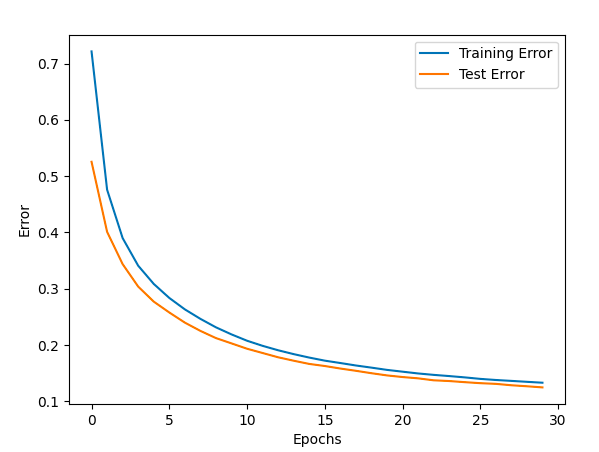
\includegraphics[scale=0.4]{d1=300e1=30}\\
  lr = 0.01 batch-size = 128 epoch = 30 \\
 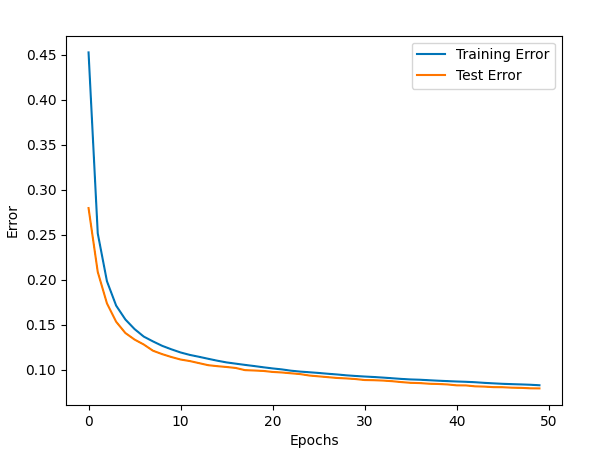
\includegraphics[scale=0.4]{d1=300e1=50}\\
  lr = 0.001 batch-size = 32 epoch = 50 \\
 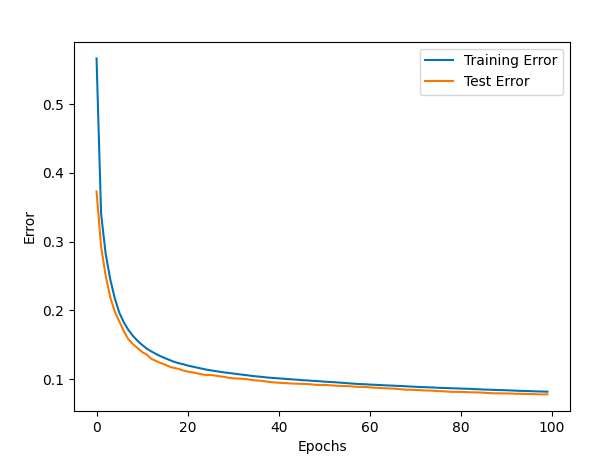
\includegraphics[scale=0.4]{d1=300e1=100}\\
  lr = 0.005 batch-size = 64 epoch = 100 \\
 
\end{center}
\end{soln}
    \item  Implement the same network in {\tt pytorch} (or any other framework). You can use all the features of the framework e.g. auto-grad etc. Evaluate it on {\tt MNIST} dataset, report test error, and learning curve. (20 pts) 
    \begin{soln}
    \begin{table}[h!]
\centering
\begin{tabular}{||c c c c c ||} 
 \hline
 d & Learning Rate & Batch Size & Epoch & Test Error \\ [0.5ex] 
 \hline\hline
 300 & 0.01 & 128 & 30 & 0.193653 \\ 
 300 & 0.001 & 32 & 50 & 0.10417 \\
 300 & 0.005 & 64 & 100 & 0.106197 \\[1ex] 
 \hline
\end{tabular}
\caption{Please find the respective graphs of each row below in order}
\label{table:1}
\end{table}
\begin{center}
For d1 = 300: \\
 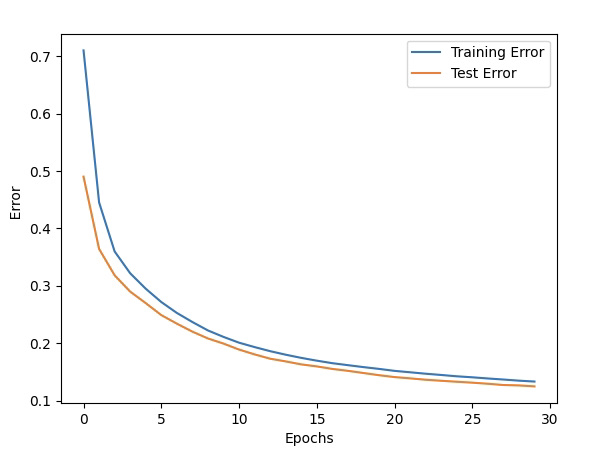
\includegraphics[scale=0.4]{d=300e=30}\\
 lr = 0.01 batch-size = 128 epoch = 30 \\
 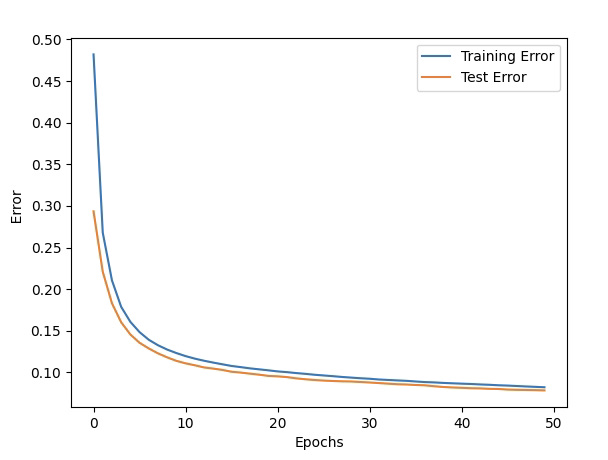
\includegraphics[scale=0.4]{d=300e=50}\\
 lr = 0.001 batch-size = 32 epoch = 50 \\
 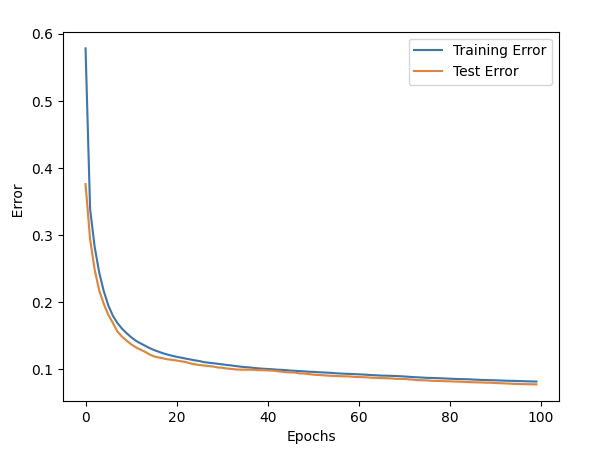
\includegraphics[scale=0.4]{d=300e=100}\\
 lr = 0.005 batch-size = 64 epoch = 100 \\
 
 \end{center}
    \end{soln}
    \item Try different weight initializations a) all weights initialized to 0, and b) Initialize the weights randomly between -1 and 1. Report test error and learning curves for both. ( You can use either of the implementations) (5 pts)
    \begin{soln}
   \\ a) Test error: 0.8865\\
     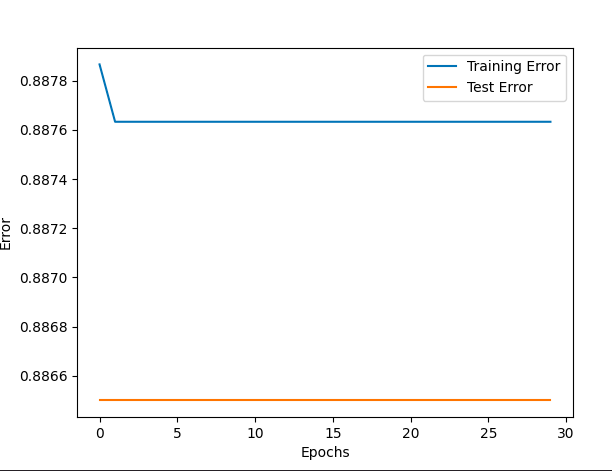
\includegraphics[scale=0.4]{w=0}\\
     b) Test error: 0.5833\\
     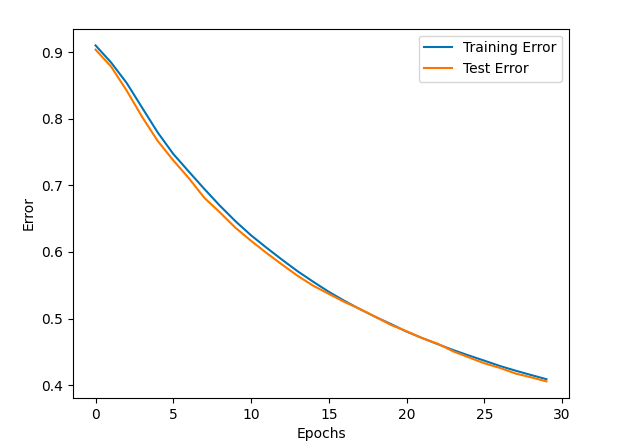
\includegraphics[scale=0.4]{w=-1..1}\\
    \end{soln}
\end{enumerate}
You should play with different hyper-parameters like learning rate, batch size, etc. For Questions 2-3; you should report the answers for at least 3 different sets of hyperparameters. You should mention the values of those along with the results. Use $d_1 = 300, d_2 = 200$. For optimization use SGD (Stochastic gradient descent) without momentum, with some batch-size say 32, 64 etc. {\tt MNIST} can be obtained from here ({\tt https://{\tt pytorch}.org/vision/ stable/datasets.html}) 

{\tt Check Piazza for a sample PyTorch project}


To load the dataset:
\begin{verbatim}
import torch
import torch.nn.functional as F
from torch.utils.data import TensorDataset, DataLoader
import torchvision

mnist_data_train = torchvision.datasets.MNIST('path/to/download',
    train=True,download=True)
data_loader = torch.utils.data.DataLoader(mnist_data,
                                          batch_size=,
                                          shuffle=True)
mnist_data_test = torchvision.datasets.MNIST('path/to/download',
    train=False,download=True)                                          
\end{verbatim}
\bibliographystyle{apalike}
\end{document}

